\documentclass[10pt]{beamer}
\usepackage[utf8]{inputenc}

\usepackage{graphicx}
\usepackage{outlines}
\usepackage[absolute,overlay]{textpos}
\usepackage{hyperref}
\hypersetup{
    colorlinks=true,
    linkcolor=blue,
    filecolor=magenta,      
    urlcolor=cyan,
    pdftitle={Overleaf Example},
    pdfpagemode=FullScreen,
    }
    
\urlstyle{same}

\mode<presentation> {
\usetheme{boxes} % When headline is wanted use Dresden theme instead
\usecolortheme{seagull}
%\logo{
\includegraphics[height=1.5cm]{ku_logo_dk}}
% \setbeamertemplate{footline}[frame number]
\setbeamertemplate{footline}{
  \hspace{1em}
  \hfill
  \insertframenumber/\inserttotalframenumber
  \vspace{1em}
  \hspace{1em}
  
\includegraphics[height=2cm]{ku_logo_dk}
  \hspace{1em}
}
\setbeamertemplate{navigation symbols}{}
\setbeamertemplate{itemize items}[square]
}


%----------------------------------------------------------------------------------------
%	TITLE PAGE
%----------------------------------------------------------------------------------------

\title[Kickstart-kursus] % bottom of every slide
  {Intro Kickstart-kursus i programmering 2023: 2} % title page

\author{\footnotesize{Daniel Spikol, The Team, \& Martin Dybdal}\\
          \footnotesize{\texttt{ds@di.ku.dk}}}

\institute {
DIKU \\ Københavns Universitet
}

\date[14. august 2023]{14.august 2023}

\begin{document}
\begin{frame}[plain]
\titlepage
\end{frame}

%%------------------------%%

\begin{frame}
\frametitle{Day 1 Part 2}
  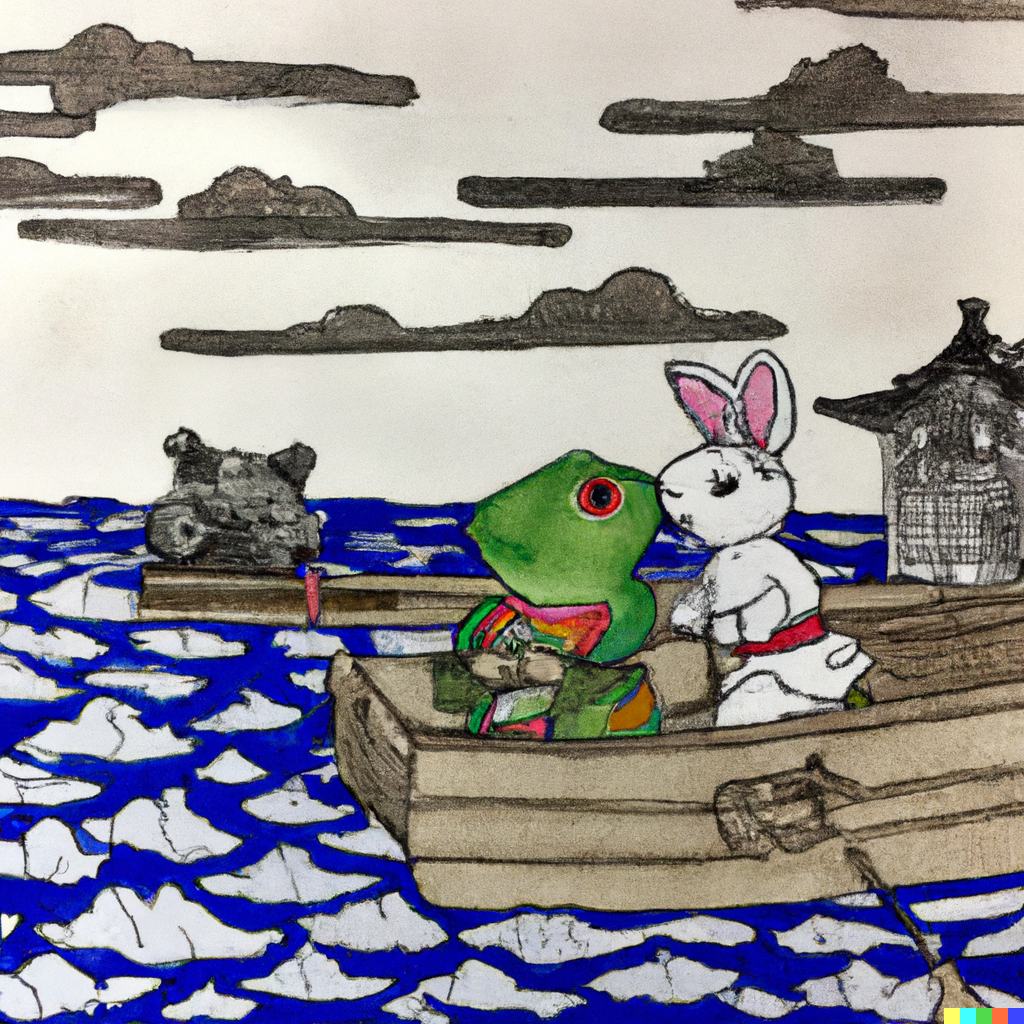
\includegraphics[height=8cm]{images/rabfro}
\end{frame}

%%------------------------%%

\begin{frame}
   \frametitle{Today's Recap}
   	\begin{itemize}
	\item Marshmallow Challenge
	\begin{itemize}
	\item constant prototyping as a problem-solving method
	\item \href{https://www.ted.com/talks/tom_wujec_build_a_tower_build_a_team?utm_campaign=tedspread&utm_medium=referral&utm_source=tedcomshare}{TED TALK Tom Wujec}
	\end{itemize}
	\item Coordinate System 
	\item Drawing with Processing
	\item Variables
	\item Functions (maybe, definitely tomorrow)
	\end{itemize}
\end{frame}

%%------------------------%%


 \begin{frame}
   \frametitle{Thinking about tomorrow}
   \begin{itemize}
   \item \href{https://en.wikipedia.org/wiki/Pair_programming}{Wikipedia: Pair Programming}
   \item \href{https://youtu.be/ET3Q6zNK3Io}{Video}
   \item \href{https://medium.com/@volkanbier_42259/how-to-put-pair-programming-into-action-ce9ebb9d711}{Good Article}
   \end{itemize}
    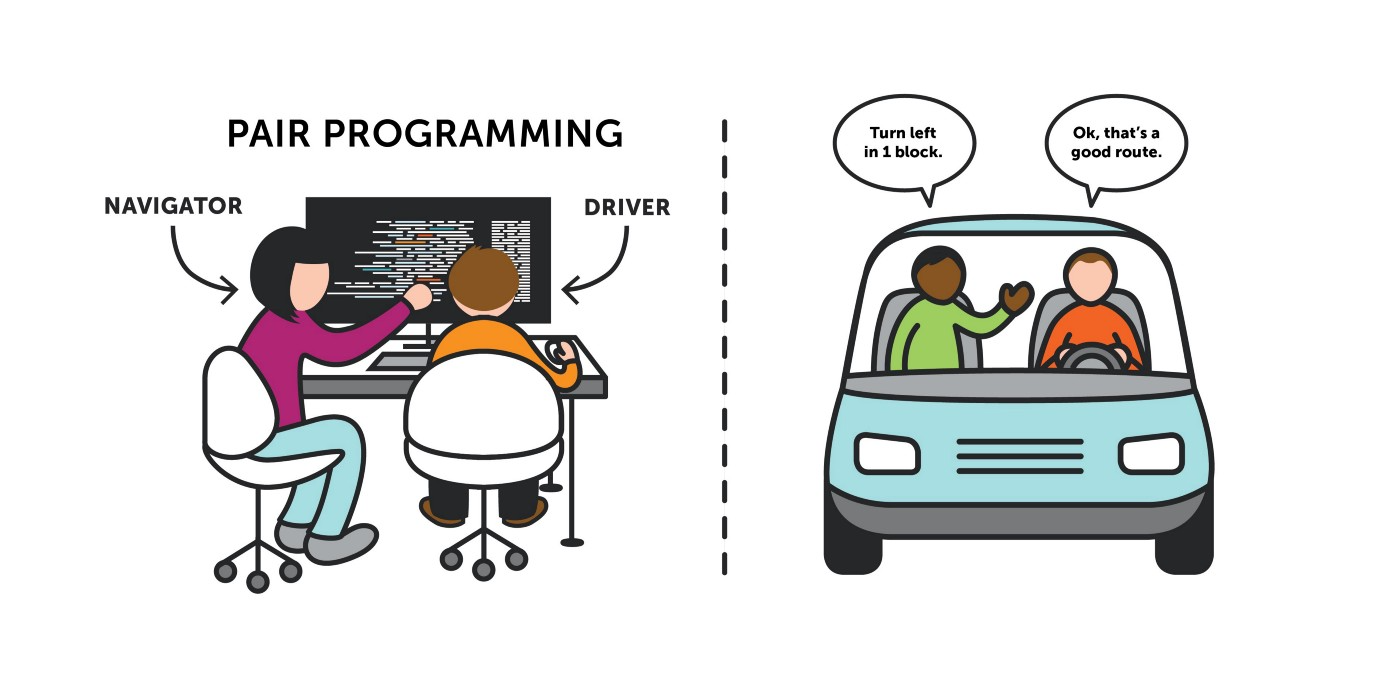
\includegraphics[width=0.9\textwidth]{images/pairpro}
\end{frame}

%%------------------------%%


 \begin{frame}
   \frametitle{Thanks}
   \begin{itemize}
  \item Tomorrow KL 9.00 sharp
  \item Aud. 06  - mini lectures on datalogy, programming, \& pair programming
   \end{itemize}
   \end{frame}

\end{document}